\documentclass[10pt,journal,compsoc]{IEEEtran}

% ---------------------------------------------------------------------------
% Submission toggle.
%   \submissiontrue  : review version -- omits biographies (the IEEE Computer
%                      Society page limit counts every page).
%   \submissionfalse : camera-ready   -- restores biographies.
% ---------------------------------------------------------------------------
\newif\ifsubmission
\submissionfalse

\usepackage{amsmath,amsfonts,amssymb}
\usepackage[noend]{algorithmic}
\renewcommand{\algorithmiccomment}[1]{\hfill$\triangleright$~#1}
\usepackage{algorithm}
\usepackage{array}
\usepackage{multirow}
\usepackage[caption=false,font=normalsize,labelfont=sf,textfont=sf]{subfig}
\usepackage{textcomp}
\usepackage{stfloats}
\usepackage{url}
\usepackage{xurl}
\usepackage{verbatim}
\usepackage{graphicx}
\usepackage{tikz}
\usetikzlibrary{arrows.meta,backgrounds,decorations.pathreplacing,
                shapes.geometric,fit,positioning,calc}
\usepackage{xcolor}
\usepackage{booktabs}
\usepackage{cite}
\hyphenation{op-tical net-works semi-conduc-tor IEEE-Xplore Technology}

\begin{document}

\title{Accelerating ALS Matrix Factorization on GPUs via Mixed-Precision Tensor Cores}

\author{Md.~Hafizur~Rahman, K.~M.~Azharul~Hasan, and Md~Mehrab~Hossain~Opi
\IEEEcompsocitemizethanks{
\IEEEcompsocthanksitem M.~H.~Rahman is with the Department of Computer Science and Engineering, Khulna University of Engineering \& Technology, Khulna 9203, Bangladesh.\protect\\
E-mail: rahman2007080@stud.kuet.ac.bd
\IEEEcompsocthanksitem K.~M.~A.~Hasan is a Professor with the Department of Computer Science and Engineering, Khulna University of Engineering \& Technology, Khulna 9203, Bangladesh.\protect\\
E-mail: az@cse.kuet.ac.bd
\IEEEcompsocthanksitem M.~M.~H.~Opi is an Assistant Professor with the Department of Computer Science and Engineering, Khulna University of Engineering \& Technology, Khulna 9203, Bangladesh.\protect\\
E-mail: opi@cse.kuet.ac.bd}}

\markboth{IEEE Transactions on Parallel and Distributed Systems}%
{Rahman \MakeLowercase{\textit{et al.}}: Accelerating ALS Matrix Factorization on GPUs via Mixed-Precision Tensor Cores}

\IEEEtitleabstractindextext{%
\begin{abstract}
Alternating least squares (ALS) is a standard method for training recommendation models, yet GPU implementations typically execute in FP32 on CUDA cores and leave tensor cores underutilized because rating matrices are sparse whereas tensor cores require dense low-precision tiles. We present APR-BALS, an adaptive-precision blocked ALS framework that overcomes this sparsity–tensor-core mismatch by routing entities according to their rating density. Entities accounting for the overwhelming majority of ratings are processed through tensor-core-based WMMA kernels using FP16 input operands with FP32 accumulation, while the sparse tail remains on a conventional FP32 path. A blocked batched Cholesky solver further prevents the solve stage from becoming a performance bottleneck. With a common binary, solver, and convergence criterion, APR-BALS achieves 4.1--14.8$\times$ speedup over an FP32 baseline on Netflix Prize data on an RTX 3060 as the latent dimension increases from 16 to 96, and up to 11.6$\times$ on MovieLens, while changing held-out RMSE by less than 0.005\%. Experiments on a Tesla T4 show the same performance trend. A three-way ablation demonstrates that reduced precision contributes at most 1.32$\times$ to the speedup, indicating that the primary performance gain comes from the WMMA tensor-core kernels. APR-BALS also achieves 3.0--6.4$\times$ lower per-iteration time than NVIDIA's \textit{cuMF\_als} GPU implementation on identical data splits. These results demonstrate that adaptive density-aware execution can effectively exploit tensor cores for sparse recommendation workloads while preserving FP32 accuracy.

\end{abstract}

\begin{IEEEkeywords}
Alternating least squares, collaborative filtering, GPU acceleration, matrix factorization, mixed precision, recommender systems, tensor cores.
\end{IEEEkeywords}}

\maketitle
\IEEEdisplaynontitleabstractindextext
\IEEEpeerreviewmaketitle

\IEEEraisesectionheading{\section{Introduction}\label{sec:intro}}

\IEEEPARstart{L}{atent-factor} collaborative filtering is among the most accurate and widely deployed techniques in recommender systems, which select, from catalogues of millions of items, the few a user is likely to value \cite{gomez2016netflix,schafer2001ecommerce}. Matrix factorization represents each user and item by a short dense vector and predicts a rating as their inner product \cite{koren2009matrix,bennett2007netflix}. Alternating least squares (ALS) trains this model by solving, in every sweep, one regularized least-squares problem per user and per item \cite{zhou2008largescale}. Each problem requires a $K \times K$ Gram matrix and an $O(K^{3})$ solve for $K$ latent factors, so the cost grows quickly with the model size: a single run on the Netflix Prize data, with 80.6 million training ratings, performs about 31~TFLOP at $K=96$.

GPU implementations of ALS exist \cite{tan2016faster,gates2015accelerating,chen2021bals}, but nearly all compute in FP32 on conventional CUDA cores. NVIDIA's data-center and RTX GPUs since Volta also carry tensor cores, which execute a dense $16 \times 16 \times 16$ half-precision multiply--accumulate as a single warp-level operation \cite{markidis2018nvidia}. The RTX~3060 used here delivers about 25.5~TFLOP/s on tensor cores with FP16 inputs and FP32 accumulation, twice its 12.7~TFLOP/s FP32 peak, and data-center parts widen this ratio considerably. Deep learning exploits these units routinely \cite{micikevicius2018mixed}; explicit-feedback ALS does not, for three reasons. First, the rating matrix is highly sparse, so Gram assembly gathers scattered factor rows while tensor cores require dense operand tiles. Second, FP16 carries only 10 mantissa bits, and its effect on recommendation accuracy under the ALS normal equations has not been measured. Third, once the Gram stage is ten times faster, the batched Cholesky solves become the critical path.

This paper addresses all three obstacles with \textit{APR-BALS} (Adaptive-Precision Blocked ALS), a CUDA implementation of explicit-feedback ALS. Rating counts follow a long-tailed distribution, with ratings distributed highly unevenly across users and items, as shown in Fig.~\ref{fig:longtail}. Because rating counts are highly skewed, entities exhibit substantially different computational workloads; consequently, a single kernel configuration cannot provide efficient execution across all entities. APR-BALS therefore sorts users and items by rating count and dispatches them in three tiers: giant and dense entities assemble their Gram matrices on tensor cores, and the sparse tail runs on a register-tiled FP32 kernel. A custom blocked Cholesky solver keeps the solve stage from absorbing the gain\cite{gates2015accelerating}. The evaluation is built on an \textit{audited baseline}: the FP32 reference shares one binary, data layout, solver, and convergence rule with the accelerated path, so every reported ratio isolates the precision dispatch. The contributions of this paper are as follows.

\begin{figure}[!t]
\centering
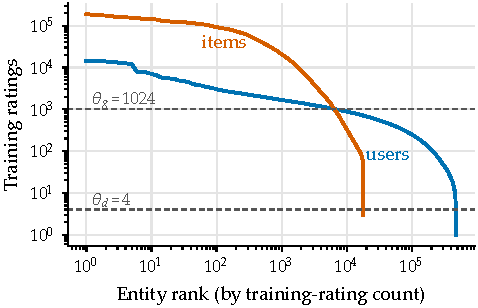
\includegraphics[width=\columnwidth]{figures/fig11_longtail.pdf}
\caption{Training ratings per user and per item in the Netflix Prize data, sorted by count. The dashed lines mark the giant and dense tier thresholds of Section~\ref{ssec:dispatch}.}
\label{fig:longtail}
\end{figure}

\begin{itemize}
\item \textbf{Density-adaptive tensor-core dispatch.} A three-tier dispatch sends more than $99.7\%$ of the training ratings to warp-level NVIDIA's Warp Matrix Multiply and Accumulate (WMMA) kernels that assemble only the upper triangle of each Gram matrix from gathered FP16 rows, with register prefetching and a multi-warp variant for very high-degree entities.
\item \textbf{A blocked batched Cholesky solver.} A $16 \times 16$-tile right-looking factorization with a fused forward solve and overlapped panel factorization runs $1.86$--$2.26\times$ faster than a tuned packed solver.
\item \textbf{An audited-baseline methodology.} A register-spill defect that crippled the FP32 baseline at $K \ge 48$, and would have inflated the speedups to $30$--$44\times$, was diagnosed and removed; no reported result uses the defective kernel. The same pitfall can affect any register-blocked Gram kernel whose accumulator footprint grows with $K^{2}$.
\item \textbf{Mechanism attribution.} A three-way ablation within one binary (FP16 WMMA, TF32 WMMA, and scalar FP32) attributes $87.8$--$99.6\%$ of the gain to the WMMA kernel at full FP32 range; reduced precision never contributes more than $1.32\times$.
\item \textbf{Comprehensive evaluation.} Speedups over the baseline reach $14.8\times$ on Netflix on an RTX~3060 and $10.8\times$ on a Tesla~T4, with test-RMSE changes below $0.005\%$ ($0.007\%$ on the T4) and run-to-run timing variation of at most $0.44\%$ over 100 runs. On identical data splits, APR-BALS is $3.0$--$6.4\times$ faster per iteration than NVIDIA's GPU-accelerated implementation of Collaborative Filtering using Alternating Least Squares (\textit{cuMF\_als})\cite{tan2016faster} and $3.4$--$4.1\times$ faster than a GPU-accelerated implementation of Collaborative Filtering using Coordinate Descent (\textit{cuMF\_CCD})\cite{yu2012scalable,nisa2017parallel}. Weighted regularization, solver-pipeline fusion, and heavy-ball momentum raise the end-to-end advantage over the baseline to $26\times$ ($19.5\times$ when iteration counts are matched.).
\end{itemize}

The evaluation covers NVIDIA Ampere and Turing GPUs and the latent dimensions $K \in \{16, 32, 48, 64, 96\}$ imposed by the WMMA tile shape; speedups on architectures with different FP16-to-FP32 throughput ratios are not established here. Section~\ref{sec:related} reviews related work, Section~\ref{sec:method} presents APR-BALS, Section~\ref{sec:eval} evaluates it against the FP32 baseline, Section~\ref{sec:extended} adds the shipped optimizations, Section~\ref{sec:external} compares it with external systems and discusses threats to validity, and Section~\ref{sec:conclusion} concludes.

\section{Related Works}
\label{sec:related}

APR-BALS draws on four lines of research: matrix factorization for collaborative filtering, GPU factorization systems, tensor-core and mixed-precision computing, and batched small-matrix solvers. Table~\ref{tab:litgap} summarizes how representative work covers the dimensions this paper combines.

\subsection{Matrix Factorization for Collaborative Filtering}

Neighbourhood methods, which compare users or items directly \cite{sarwar2001item}, gave way to latent-factor models after the Netflix Prize released about 100 million ratings \cite{bennett2007netflix}. Koren et al. showed that regularized matrix factorization outperforms neighbourhood approaches and scales to industrial data \cite{koren2009matrix}, and Later models extended the same factorization framework by incorporating neighborhood effects and implicit feedback signals\cite{koren2008factorization}. The model is trained mainly by stochastic gradient descent (SGD), which is cheap per update but inherently sequential, or by ALS \cite{zhou2008largescale}, which costs a Gram matrix and a Cholesky solve per entity but parallelizes naturally because each entity's subproblem is independent. ALS also extends to the confidence-weighted implicit-feedback objective of Hu et al.\ \cite{hu2008collaborative}, and its sweep count can be reduced by extrapolation, as shown for tensor decomposition \cite{ma2022pairwise,evans2023blockwise}; the momentum scheme of Section~\ref{sec:extended} applies the same principle to matrix factorization. We target explicit-feedback ALS because its dense per-entity subproblems expose structure that tensor cores can consume, and we evaluate on the Netflix and MovieLens \cite{harper2016movielens} benchmarks.

\subsection{Parallel and GPU-Accelerated Factorization}

On CPUs, Hogwild!, a parallel SGD (Stochastic Gradient Descent) approach, runs SGD largely lock-free \cite{recht2011hogwild}, DSGD partitions the rating matrix for distributed SGD \cite{gemulla2011large}, and enhanced Coordinate Descent (CCD++) reformulates training as cache-friendly coordinate descent \cite{yu2012scalable}. These systems scale out but do not raise per-operation throughput. On GPUs, the leading explicit-ALS system is \textit{cuMF\_als}, which tiles Gram assembly through registers and shared memory \cite{tan2016faster}; it can store the Conjugate Gradient (CG)  system matrix in FP16 to save bandwidth but computes on CUDA cores. The same project, the GPU CCD++,  provides \textit{cuMF\_SGD} \cite{xie2017cumf} and \textit{cuMF\_CCD}. \cite{nisa2017parallel}. Gates et al.\ accelerated implicit-feedback ALS with batched kernels and autotuning \cite{gates2015accelerating}; because that objective combines a dense Gram term shared by all users with a sparse per-user correction. Chen et al.\ proposed BALS, a blocked ALS built on a tiled sparse format \cite{chen2021bals}, which serves as the storage baseline of our scalar path. As Volkov and Demmel showed, performance depends on matching kernel structure to the microarchitecture \cite{volkov2008benchmarking}, which on current GPUs includes tensor cores.
%Table~\ref{tab:litgap} shows a summary of coverage of key issues of important related works.

\begin{table}[!t]
\caption{Coverage of Key Dimensions by Representative Related Work}
\label{tab:litgap}
\centering
\footnotesize
\renewcommand{\arraystretch}{1.15}
\setlength{\tabcolsep}{2.2pt}
\begin{tabular}{lccccc}
\toprule
\textbf{Work} & \textbf{ALS/MF} & \textbf{GPU} & \textbf{Tensor} & \textbf{Sparse-} & \textbf{Accuracy} \\
 & & & \textbf{cores} & \textbf{aware} & \textbf{check} \\
\midrule
Zhou et al.~\cite{zhou2008largescale}            & ALS    & No  & No  & Yes & Yes \\
Tan et al.~\cite{tan2016faster}                  & ALS    & Yes & No  & Yes & Yes \\
Xie et al.~\cite{xie2017cumf}                    & SGD    & Yes & No  & Yes & Yes \\
Gates et al.~\cite{gates2015accelerating}        & ALS    & Yes & No  & Partial & Yes \\
Chen et al.~\cite{chen2021bals}                  & ALS    & Yes & No  & Yes & Yes \\
Markidis et al.~\cite{markidis2018nvidia}        & No     & Yes & Yes & No  & Kernel \\
Haidar et al.~\cite{haidar2018harnessing}        & No     & Yes & Yes & No  & Solver \\
Zachariadis et al.~\cite{zachariadis2020accelerating} & No & Yes & Yes & Yes & Kernel \\
Fan et al.~\cite{fan2024dtcspmm}                 & No     & Yes & Yes & Yes & Kernel \\
Abdelfattah et al.~\cite{abdelfattah2017factorization} & No & Yes & No & No & Solver \\
\midrule
\textbf{APR-BALS (this work)} & \textbf{ALS} & \textbf{Yes} & \textbf{Yes} & \textbf{Yes} & \textbf{End-to-end} \\
\bottomrule
\end{tabular}
\end{table}

\subsection{Tensor Cores and Mixed-Precision Computing}

Tensor cores perform a $16\times16 \times16$ matrix multiply accumulate per warp-level instruction with FP16 inputs and FP32 accumulation. Their throughput, programmability, and rounding behaviour have been characterized by Markidis et al.\cite{markidis2018nvidia} and by microbenchmark studies through the Hopper generation\cite{jia2018dissecting,luo2024hopper}, and the WMMA interface is specified in the CUDA documentation \cite{nvidia2023cuda}. Blanchard et al.\ bounded the rounding error of the block fused multiply add these units implement, showing that FP32 accumulation of FP16 products is far more accurate than pure FP16 arithmetic\cite{blanchard2020mixed}; Higham and Mary survey the mixed-precision algorithms built on such guarantees \cite{higham2002accuracy,higham2022mixed}. Mixed precision is established in deep learning \cite{micikevicius2018mixed} and in dense solvers, where tensor-core iterative refinement solves FP64 systems up to $4\times$ faster \cite{haidar2018harnessing} and least-squares problems admit several refinement strategies \cite{carson2025comparison}. Those methods recover a high-precision solution from a low-precision factorization; we ask instead whether the ALS normal equations tolerate low-precision \textit{formation} without refinement. For sparse computations, Zachariadis et al.\ dispatched dense sub-blocks of sparse matrix matrix products to tensor cores \cite{zachariadis2020accelerating}, and recent systems refine this approach through data movement optimization \cite{fan2024dtcspmm}, format and pipeline co-design \cite{zhao2025accspmm}, support for unstructured patterns \cite{okanovic2024unstructured}, and block-density transformations \cite{dong2026blocksmith}. Each optimizes a single sparse kernel in isolation; none embeds it in a training loop or reports the accuracy of the resulting model.

\subsection{Batched Small-Matrix Solvers}

Each ALS half-iteration produces hundreds of thousands of independent $K\times K$ symmetric positive-definite systems. Abdelfattah et al. analyzed the occupancy, register-pressure, and memory-layout trade-offs of factorizing many small matrices on GPUs \cite{abdelfattah2017factorization}, and Luszczek et al. proposed interfaces for batched sparse and mixed-precision solvers embedded in larger applications \cite{luszczek2024batched}. Our solver adapts the classical blocked right-looking factorization \cite{golub2013matrix} to the shared-memory capacity and synchronization model of a single streaming multiprocessor.

%\subsection{Summary and Research Gap}

Existing GPU ALS systems compute on FP32 CUDA cores. Tensor-core studies deliver fast dense and sparse kernels but close no training loop around them and do not assess model accuracy, and batched-solver studies optimize the factorization apart from the pipeline that feeds it. No prior system trains explicit-feedback ALS on tensor cores with a density-adaptive precision dispatch and shows, against an audited FP32 baseline under identical conditions, that the end-to-end accuracy cost is negligible.

\section{The APR-BALS System}
\label{sec:method}

\subsection{ALS Formulation and Cost Model}
\label{ssec:formulation}

Let $R \in \mathbb{R}^{m \times n}$ hold the ratings of $m$ users on $n$ items, and let $\Omega$ be the set of observed positions. A rank-$K$ model $R \approx XY^{\mathsf{T}}$ assigns a latent vector $\mathbf{x}_u \in \mathbb{R}^{K}$ to each user and $\mathbf{y}_i \in \mathbb{R}^{K}$ to each item, and predicts $\hat{r}_{ui} = \mathbf{x}_u^{\mathsf{T}}\mathbf{y}_i$. Training minimizes the regularized squared error
\begin{equation}
\min_{X,Y} \sum_{(u,i)\in\Omega} \bigl( r_{ui} - \mathbf{x}_u^{\mathsf{T}} \mathbf{y}_i \bigr)^{2}
+ \lambda \Bigl( \sum_{u} n_u \lVert \mathbf{x}_u \rVert^{2} + \sum_{i} n_i \lVert \mathbf{y}_i \rVert^{2} \Bigr),
\label{eq:mf_objective}
\end{equation}
where $n_u$ and $n_i$ are training-rating counts. This per-entity weighting is the ALS-WR regularizer of Zhou et al.\ \cite{zhou2008largescale}; Section~\ref{ssec:weightedlambda} explains why we prefer it to a uniform penalty. With $Y$ fixed, each user's subproblem is a ridge regression with the normal equation
\begin{equation}
\bigl( \underbrace{Y_{\Omega(u)}^{\mathsf{T}} Y_{\Omega(u)}}_{A_u} + \lambda n_u I \bigr)\, \mathbf{x}_u = \underbrace{Y_{\Omega(u)}^{\mathsf{T}} \mathbf{r}_u}_{\mathbf{b}_u},
\label{eq:als_update}
\end{equation}
where $Y_{\Omega(u)}$ stacks the factor rows of the items rated by $u$. The system is symmetric positive definite and is solved by Cholesky factorization \cite{golub2013matrix}. The item side is symmetric, and one ALS sweep solves all users and then all items.

Each half-sweep has two stages. Gram assembly forms $A_u$ and $\mathbf{b}_u$ for every entity; exploiting the symmetry of $A_u$, it costs
\begin{equation}
F_{\text{gram}} = 2\,|\Omega| \left( \tfrac{K(K+1)}{2} + K \right)
\label{eq:gram_flops}
\end{equation}
floating-point operations per side. The solve stage then factorizes $m$ (or $n$) independent $K \times K$ systems at about $K^{3}/3$ operations each. On Netflix at $K=64$, Gram assembly performs about 690~GFLOP per sweep, over an order of magnitude more than the solves, and the FP32 baseline\cite{chen2021bals} spends $96\%$ of its time there. Once Gram assembly is accelerated $10 \times$, the linear-system solve emerges as the dominant runtime component. APR-BALS therefore treats the solver as a first-class optimization target.

\textbf{Error model.} FP16 operands with FP32 accumulation admit a tighter bound than generic mixed precision. The WMMA path forms $A_u$ from $s = \lceil n_u/16 \rceil$ rank-16 updates. The product of two FP16 values is exact in FP32, because two 11-bit significands need at most 22 of FP32's 24 bits. Two error sources remain: rounding the operands to FP16, bounded by the unit roundoff $u_{16} = 2^{-11}$, and FP32 accumulation over $s$ terms, bounded by $\gamma_s^{(32)} = s u_{32}/(1 - s u_{32})$ with $u_{32} = 2^{-24}$ \cite{blanchard2020mixed,higham2002accuracy}. Hence
\begin{equation}
|\hat{A}_{pq} - A_{pq}| \;\lesssim\; \bigl( 2u_{16} + \gamma_s^{(32)} \bigr)\, \lVert Y_{\Omega(u)} \rVert_F^{2}.
\label{eq:error_bound}
\end{equation}
The heaviest Netflix user has 14{,}123 training ratings, so $s \le 883$ and $\gamma_s^{(32)} \le 5.3 \times 10^{-5}$, about $19\times$ below $2u_{16} \approx 9.8 \times 10^{-4}$. The heaviest item has 187{,}512 ratings, but the giant kernel splits it across four warps (Section~\ref{ssec:wmma}), so each accumulates at most 2{,}930 terms and $\gamma_s^{(32)} \le 1.8 \times 10^{-4}$, still $5.6\times$ below the operand term. For every entity, the error is therefore dominated by operand rounding, which does not depend on degree, so a single dispatch rule is safe across a long-tailed degree distribution. With FP16 accumulation the bound would be $0.76$ for the heaviest user and meaningless for the heaviest item, which is why all accumulation stays in FP32. The bound ignores the 16-term accumulation inside each WMMA instruction ($\gamma_{16}^{(32)} \approx 9.5 \times 10^{-7}$) and assumes round-to-nearest, which tensor cores do not implement exactly \cite{markidis2018nvidia}. Because $\hat{A}_u$ and $\hat{\mathbf{b}}_u$ come from the same rounded rows, the WMMA path solves, up to accumulation error, the exact ridge problem on slightly perturbed features, and $\hat{A}_u$ stays positive semidefinite. Under the weighted regularizer, $\kappa(A_u + \lambda n_u I) \le 1 + \max_i \lVert \mathbf{y}_i \rVert^{2}/\lambda$ for every degree, so the solve amplifies the Gram error by a bounded factor, and Section~\ref{ssec:main_results} measures the end effect. FP16's range limit (65{,}504) is separate (Section~\ref{ssec:momentum}).

\subsection{System Overview}
\label{ssec:framework}

Fig.~\ref{fig:framework} shows the three stages of APR-BALS, and Algorithm~\ref{alg:training} gives the training loop. Offline preprocessing sorts users and items by rating count, applies a random 80/20 train/test split, and writes both into a frozen binary file; every system evaluated in this paper reads the same file. At start-up, the host builds the scalar path's tiled storage and each side's tier boundaries $N_g \le N_d$ (Section~\ref{ssec:dispatch}).

\begin{algorithm}[!t]
\caption{APR-BALS training loop (host side)}
\label{alg:training}
\small
\begin{algorithmic}[1]
\REQUIRE frequency-sorted ratings; tier boundaries $N_g \le N_d$ per side; $X, Y \sim U(0, 0.2)$
\FOR{$t = 1$ \TO $50$}
  \FORALL{$(Z, W) \in \{(X, Y), (Y, X)\}$}
    \STATE $\widehat{W} \gets \mathrm{fp16}(W)$ \COMMENT{solve $Z$ with $W$ fixed}
    \FORALL{batches $B$ of 60{,}000 entities}
      \STATE \textbf{stream 1:} wait until Gram buffer $B \bmod 2$ is free \label{alg:tr:wait}
      \STATE \quad \textsc{Giant}$(B \cap [0, N_g))$, \textsc{Dense}$(B \cap [N_g, N_d))$
      \STATE \quad \textsc{Scalar}$(B \cap [N_d, \infty))$ \COMMENT{$A_u$, $\mathbf{b}_u$ in FP32}
      \STATE \textbf{stream 2:} after stream 1, solve \eqref{eq:als_update} for all $u \in B$ \label{alg:tr:solve}
    \ENDFOR
    \STATE $Z \gets Z + \beta (Z - Z_{\text{prev}})$ \COMMENT{shipped only}
  \ENDFOR
  \IF{$t \bmod 5 = 0$}
    \STATE $r \gets \textsc{TrainRMSE}(X, Y)$
    \STATE \textbf{if} $|r - r_{\text{prev}}| < 10^{-3}$ \textbf{then stop}; $r_{\text{prev}} \gets r$
  \ENDIF
\ENDFOR
\end{algorithmic}
\end{algorithm}

\begin{figure}[!t]
\centering
% Fig. 2 -- APR-BALS framework, drawn at one-column width (3.5 in).
% IEEE: figure type ~9-10 pt at print size, never below 6 pt.
% Box text is \footnotesize (8 pt); labels are \scriptsize (7 pt).
% Sans-serif text, black outlines, one fill colour per execution unit:
% gold = tensor cores, blue = CUDA cores, green = solver, grey = set-up.
\definecolor{fwTC}{HTML}{FFE699}
\definecolor{fwTCbar}{HTML}{F4B400}
\definecolor{fwSC}{HTML}{DDEBF7}
\definecolor{fwSCbar}{HTML}{9DC3E6}
\definecolor{fwSolve}{HTML}{C6E0B4}
\definecolor{fwSetup}{HTML}{EDEDED}
\begin{tikzpicture}[
    font=\sffamily\footnotesize,
    >={Stealth[length=3.6pt, width=3.2pt]},
    box/.style={draw=black!85, line width=0.6pt, align=center, inner sep=1.5pt,
                minimum height=8mm},
    setup/.style={box, fill=fwSetup},
    tier/.style={box, minimum width=26mm, minimum height=8.5mm},
    bar/.style={draw=black!85, line width=0.6pt, font=\sffamily\scriptsize\bfseries,
                inner sep=0pt, minimum height=4mm, align=center},
    stage/.style={box, fill=white},
    tag/.style={draw=black!70, fill=white, rounded corners=3.5pt, line width=0.4pt,
                font=\scriptsize, inner sep=1.2pt},
    lbl/.style={font=\sffamily\scriptsize, text=black!80, inner sep=1pt},
    dot/.style={circle, fill=black, inner sep=0pt, minimum size=2.4pt},
    flow/.style={->, line width=0.6pt},
    wire/.style={line width=0.6pt}]

% Row 1: set-up (runs once)
\node[setup, minimum width=40mm] (pre) at (0,0)
  {\textbf{Offline:} frequency sort,\\frozen 80/20 train/test split};
\node[setup, minimum width=38mm, right=4mm of pre] (host)
  {\textbf{Host:} tiled storage,\\tier split by $\theta_g$ and $\theta_d$};
\draw[flow] (pre) -- (host);

% Row 2: three-tier Gram assembly, standing on an execution-unit bar
\node[tier, fill=fwTC, below=14mm of pre.south west, anchor=north west] (giant)
  {\strut\textbf{Giant tier}\\\strut 4-warp WMMA};
\node[tier, fill=fwTC, right=1.5mm of giant] (dense)
  {\strut\textbf{Dense tier}\\\strut 1-warp WMMA};
\node[tier, fill=fwSC, right=1.5mm of dense] (sparse)
  {\strut\textbf{Sparse tail}\\\strut tiled scalar kernel};
\node[bar, fill=fwTCbar, anchor=north west, minimum width=53.5mm]
  (tcbar) at (giant.south west) {Tensor cores: FP16 in, FP32 accumulate};
\node[bar, fill=fwSCbar, anchor=north west, minimum width=26mm]
  (scbar) at (sparse.south west) {CUDA cores: FP32};

% Dispatch bus; each drop carries its routing rule (Eq. tier_def)
\coordinate (disp) at ($(giant.north)+(0,5mm)$);
\coordinate (ret)  at ($(sparse.east)+(3.2mm,0)$);
\draw[wire] (giant.north |- disp) -- (ret |- disp);
\draw[flow] (host.south) -- (host.south |- disp);
\node[dot] at (host.south |- disp) {};
\draw[flow] (giant.north |- disp)  -- node[tag] {$n_u \ge \theta_g$} (giant.north);
\draw[flow] (dense.north |- disp)  -- node[tag] {$\theta_d \le n_u < \theta_g$} (dense.north);
\draw[flow] (sparse.north |- disp) -- node[tag] {$n_u < \theta_d$} (sparse.north);

% Row 3: merge, solve, update, check
\node[stage, below=6.5mm of tcbar.south west, anchor=north west] (gram)
  {FP32 Gram\\$A_u$, $\mathbf{b}_u$};
\node[box, fill=fwSolve, right=2.5mm of gram] (chol)
  {\textbf{Blocked batched}\\\textbf{Cholesky}};
\node[stage, dashed, right=2.5mm of chol] (mom)
  {Heavy-ball\\momentum};
\node[stage, right=2.5mm of mom] (rmse)
  {Train RMSE\\every 5 sweeps};
\draw[flow] (gram) -- (chol);
\draw[flow] (chol) -- (mom);
\draw[flow] (mom) -- (rmse);

% Both bars feed the FP32 Gram buffers
\coordinate (bus) at ($(tcbar.south)+(0,-3mm)$);
\draw[wire] (tcbar.south) -- (tcbar.south |- bus);
\draw[wire] (scbar.south) -- (scbar.south |- bus);
\draw[wire] (scbar.south |- bus) -- (gram.north |- bus);
\draw[flow] (gram.north |- bus) -- (gram.north);

% Loop back to the dispatch bus: next batch, then the other side
\draw[flow] (rmse.east) -| (ret |- disp);
\node[lbl, rotate=90, anchor=south] at ($(ret |- scbar.south)+(0,0)$) {next batch};

% Training-loop frame with its legend on the top edge
\coordinate (top) at ($(disp)+(0,3mm)$);
\begin{scope}[on background layer]
\node[draw=black!45, dashed, rounded corners=2pt, inner sep=1.2mm, line width=0.5pt,
      fit=(giant)(sparse)(gram)(rmse)(ret)(top)] (loop) {};
\end{scope}
\node[lbl, fill=white, anchor=west, inner sep=1.2pt] at ($(loop.north west)+(2mm,0)$)
  {\textbf{Training loop}};
\end{tikzpicture}

\caption{Overview of APR-BALS. The host routes each entity by its rating count $n_u$ (Eq.~\ref{eq:tier_def}) to two tensor-core tiers or a scalar FP32 tier. All tiers write FP32 Gram matrices, which a blocked batched Cholesky kernel solves. Each loop pass handles one batch of 60{,}000 entities, and user and item sides alternate. The dashed momentum step belongs to the shipped configuration only. The FP32 baseline runs the same binary with every entity routed to the scalar tier.}
\label{fig:framework}
\end{figure}

\subsection{Frequency Sorting and Tier Dispatch}
\label{ssec:dispatch}

Frequency sorting renumbers users and items in decreasing order of rating count. The sort runs once offline, and afterwards every tier is a contiguous index range rather than a scatter list: the giant tier is $[0, N_g]$, the dense tier $[N_g, N_d]$, and the sparse tier the rest. With $n_u$ the training-rating count of entity $u$, the dispatch is
\begin{equation}
\text{tier}(u) =
\begin{cases}
\text{giant}, & n_u \ge \theta_g, \\
\text{dense}, & \theta_d \le n_u < \theta_g, \\
\text{sparse}, & n_u < \theta_d .
\end{cases}
\label{eq:tier_def}
\end{equation}
The dense threshold is $\theta_d = 4$. The WMMA kernels consume ratings in chunks of 16, and an entity with fewer than four ratings fills less than a quarter of one chunk. The giant threshold is tuned per dataset (1024 for Netflix, 512 for MovieLens); Section~\ref{ssec:sensitivity} shows that performance is flat in $\theta_g$ but sensitive to $\theta_d$. Tier boundaries are rounded to multiples of 32 so that they align with tile rows of the scalar path.

The split is highly skewed. On Netflix, the sparse tier receives $7{,}229$ users ($1.5\%$) but only $0.016\%$ of the training ratings. Across all datasets and both sides, the tensor-core tiers receive at least $99.77\%$ of the training ratings. The numerous but nearly empty sparse tail stays on CUDA cores in the tiled format of BALS \cite{chen2021bals}, which stages each 32-row tile's distinct feature rows in shared memory once; tiles with density $d_t \ge 10^{-3}$ stage them in FP16 but compute in FP32.

\subsection{Tensor-Core Gram Kernels}
\label{ssec:wmma}

Algorithm~\ref{alg:wmma} shows both tensor-core kernels. They read the FP16 copy $\widehat{W}$ of the fixed factor matrix made at the start of the half-sweep. In the \textit{dense kernel} ($P=1$), one warp processes one entity. The warp gathers the FP16 feature rows of 16 rated items at a time into a $16 \times K$ shared-memory tile $S$ using 16-byte loads (line~\ref{alg:wm:stage}). It then adds $S^{\mathsf{T}} S$ to the Gram matrix one $16 \times 16$ block at a time (Fig.~\ref{fig:wmma}). Computing only the upper triangle takes
\begin{equation}
N_{\text{frag}} = \frac{K_T (K_T + 1)}{2}, \qquad K_T = K/16,
\label{eq:frag_count}
\end{equation}
WMMA operations per chunk (line~\ref{alg:wm:mma}), which saves $25\%$ of the tensor-core work at $K=32$ and $42\%$ at $K=96$. The accumulators stay in FP32 register fragments for the entity's entire rating list, and $\mathbf{b}_u$ is accumulated in the same pass. For $K \le 48$, a register double buffer prefetches the next chunk; at larger $K$ no registers remain for it.

The \textit{giant kernel} ($P=4$) handles entities with thousands of ratings, which would otherwise keep one warp busy while the rest of the GPU idles. Its four warps take interleaved chunks of the same entity and reduce their partial matrices through shared memory (line~\ref{alg:wm:reduce}). Neither kernel uses atomic operations, so both are deterministic.

\begin{figure}[!t]
\centering
% Dense-tier WMMA Gram assembly, one chunk at K=64 (K_T=4), one-column width.
% Same type sizes as Fig. 2: \footnotesize (8 pt) labels, \scriptsize (7 pt) notes.
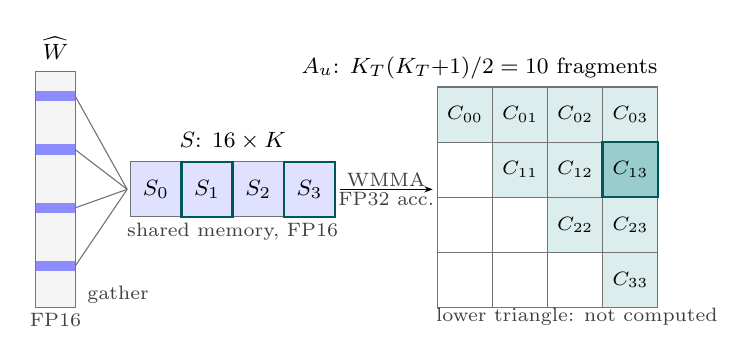
\begin{tikzpicture}[
    font=\footnotesize, x=1mm, y=1mm,
    >={Stealth[length=3pt]},
    cell/.style={draw=black!55, line width=0.4pt},
    hot/.style={line width=0.9pt, draw=teal!70!black},
    note/.style={font=\scriptsize, text=black!75, inner sep=0.8pt},
    flow/.style={->, line width=0.5pt}]

% --- FP16 factor matrix W-hat; four of the 16 gathered rows highlighted
\draw[cell, fill=black!4] (0,0) rectangle (5,30);
\foreach \y in {26.2, 19.4, 12.0, 4.6}
  \fill[blue!45] (0,\y) rectangle (5,\y+1.3);
\node[anchor=south] at (2.5,30.3) {$\widehat{W}$};
\node[note, anchor=north] at (2.5,-0.4) {FP16};
\foreach \y in {26.85, 20.05, 12.65, 5.25}
  \draw[line width=0.4pt, black!55] (5,\y) -- (11.6,15);
\node[note, anchor=south west] at (6.2,0.2) {gather};

% --- shared-memory tile S = 16 x K as four 16x16 column blocks
\foreach \m in {0,1,2,3} {
  \draw[cell, fill=blue!12] (12+6.5*\m,11.5) rectangle (18.5+6.5*\m,18.5);
  \node at (15.25+6.5*\m,15) {$S_{\m}$};
}
\draw[hot] (18.5,11.5) rectangle (25,18.5);
\draw[hot] (31.5,11.5) rectangle (38,18.5);
\node[anchor=south] at (25,18.8) {$S$: $16 \times K$};
\node[note, anchor=north] at (25,11.1) {shared memory, FP16};

% --- Gram matrix A_u as 4x4 fragments; upper triangle held in FP32 registers
\foreach \m in {0,1,2,3}
  \foreach \n in {0,1,2,3} {
    \pgfmathtruncatemacro{\up}{\n >= \m ? 1 : 0}
    \ifnum\up=1
      \draw[cell, fill=teal!14] (51+7*\n,28-7*\m) rectangle (58+7*\n,21-7*\m);
      \node[font=\scriptsize] at (54.5+7*\n,24.5-7*\m) {$C_{\m\n}$};
    \else
      \draw[cell, fill=white] (51+7*\n,28-7*\m) rectangle (58+7*\n,21-7*\m);
    \fi
  }
\draw[hot, fill=teal!40] (72,21) rectangle (79,14);
\node[font=\scriptsize] at (75.5,17.5) {$C_{13}$};
\node[anchor=south east, inner sep=0pt] at (79,29) {$A_u$: $K_T(K_T{+}1)/2 = 10$ fragments};
\node[note, anchor=north west] at (50.5,0.3) {lower triangle: not computed};

\draw[flow] (38.6,15) -- node[note, above] {WMMA} node[note, below] {FP32 acc.} (50.4,15);
\end{tikzpicture}

\caption{Dense-tier Gram assembly for one 16-rating chunk at $K=64$ ($K_T=4$). The warp gathers the FP16 factor rows of the chunk's items into $S$ and updates the ten upper-triangle fragments $C_{mn}$ of $A_u$ in FP32 registers. The highlighted update is $C_{13} \mathrel{+}= S_1^{\mathsf{T}} S_3$ (Algorithm~\ref{alg:wmma}, lines~\ref{alg:wm:stage}--\ref{alg:wm:mma}).}
\label{fig:wmma}
\end{figure}

\begin{algorithm}[!t]
\caption{Tensor-core Gram assembly for one entity $u$. $S_m$ is the $m$-th block of 16 columns of $S$}
\label{alg:wmma}
\small
\begin{algorithmic}[1]
\REQUIRE $\widehat{W}$ (FP16); ratings $(j_k, r_k)$, $0 \le k < n_u$; $P$ warps per entity (dense: 1, giant: 4)
\FORALL{warps $p = 0, \dots, P-1$ \textbf{in parallel}}
  \STATE $C_{mn} \gets 0$ for $0 \le m \le n < K_T$; $\mathbf{c} \gets \mathbf{0}$ \COMMENT{FP32}
  \FOR{$k_0 = 16p$ \TO $n_u - 1$ \textbf{step} $16P$}
    \STATE $S \gets \widehat{W}[j_{k_0}, \dots, j_{k_0+15}]$ \COMMENT{$16 \times K$, zero-padded} \label{alg:wm:stage}
    \FOR{$m = 0$ \TO $K_T - 1$; $n = m$ \TO $K_T - 1$}
      \STATE $C_{mn} \gets C_{mn} + S_m^{\mathsf{T}} S_n$ \COMMENT{one WMMA, FP32 acc.} \label{alg:wm:mma}
    \ENDFOR
    \STATE $\mathbf{c} \gets \mathbf{c} + S^{\mathsf{T}} (r_{k_0}, \dots, r_{k_0+15})^{\mathsf{T}}$
  \ENDFOR
\ENDFOR
\STATE \textbf{if} $P > 1$: sum $C_{mn}$, $\mathbf{c}$ over warps in shared memory \label{alg:wm:reduce}
\STATE write $C_{mn}$ to the upper triangle of $A_u$ and $\mathbf{c}$ to $\mathbf{b}_u$
\end{algorithmic}
\end{algorithm}

\subsection{Scalar Kernel and Baseline Audit}
\label{ssec:scalar}

The scalar kernel assembles Gram contributions tile by tile. A thread block stages a tile's feature rows into shared memory, and each thread accumulates an $R \times R$ register block of the $K \times K$ output, with $R=3$ for $K \in \{48, 96\}$ and $R=2$ otherwise. Contributions are flushed to the Gram buffer with atomic additions. The same kernel, with every entity routed to it, is the FP32 baseline for every speedup, so its quality is critical.

An early version of this kernel was defective. One thread block covered a full 32-row tile row, so each thread held $K^{2}/32$ persistent accumulators. Under the 64-register limit required for full occupancy, these spilled to local memory at $K \ge 48$. The spill traffic throttled the baseline to 51--63~GFLOP/s and inflated the apparent speedups to 30--44$\times$. The fix, \textit{row splitting}, divides each tile row among $G$ sibling blocks ($G = 1, 2, 4, 8, 8$ for the five values of $K$), which reduces the per-thread accumulator set $G$-fold without changing the arithmetic order (Fig.~\ref{fig:rowsplit}, Table~\ref{tab:baselineaudit}).

\begin{figure}[!t]
\centering
% Row splitting in the scalar baseline kernel, K=64 (G=8), one-column width.
% Numbers: per-thread accumulators = K^2/(32G) (FIXLOG 07-04b; 1024-thread blocks,
% R x R register tiles); K=64 -> 128 before (G=1), 16 after (G=8).
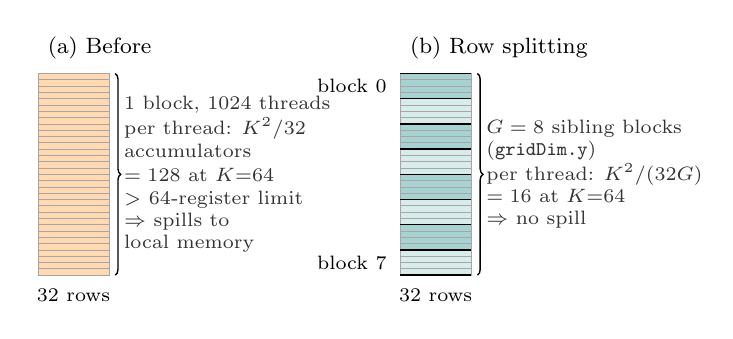
\begin{tikzpicture}[
    font=\footnotesize, x=1mm, y=1mm,
    row/.style={draw=black!35, line width=0.25pt},
    note/.style={font=\scriptsize, text=black!80, inner sep=0.8pt, align=left},
    brace/.style={decorate, decoration={brace, amplitude=2pt}, line width=0.5pt}]

% (a) defective: one block owns the whole 32-row tile row
\node[anchor=south west] at (0,27.4) {(a) Before};
\foreach \r in {0,...,31}
  \draw[row, fill=orange!30] (0,26-0.8*\r) rectangle (9,26.8-0.8*\r);
\draw[brace] (9.8,26.8) -- (9.8,1.2) node[midway, right=2.2pt, note]
  {1 block, 1024 threads\\[1pt]per thread: $K^2/32$\\accumulators\\[1pt]$= 128$ at $K{=}64$\\$>$ 64-register limit\\$\Rightarrow$ spills to\\local memory};

% (b) row splitting: G = 8 sibling blocks, 4 rows each
\node[anchor=south west] at (46,27.4) {(b) Row splitting};
\foreach \g in {0,...,7}
  \foreach \r in {0,...,3} {
    \pgfmathtruncatemacro{\shade}{mod(\g,2) == 0 ? 35 : 15}
    \draw[row, fill=teal!\shade] (46,26-3.2*\g-0.8*\r) rectangle (55,26.8-3.2*\g-0.8*\r);
  }
\foreach \g in {0,...,7}
  \draw[line width=0.5pt] (46,26.8-3.2*\g) -- (55,26.8-3.2*\g);
\draw[line width=0.5pt] (46,1.2) -- (55,1.2);
\node[font=\scriptsize, anchor=east] at (45.5,25.2) {block 0};
\node[font=\scriptsize, anchor=east] at (45.5,2.8) {block 7};
\draw[brace] (55.8,26.8) -- (55.8,1.2) node[midway, right=2.2pt, note]
  {$G = 8$ sibling blocks\\(\texttt{gridDim.y})\\[1pt]per thread: $K^2/(32G)$\\$= 16$ at $K{=}64$\\$\Rightarrow$ no spill};
\node[font=\scriptsize, anchor=north] at (4.5,0.7) {32 rows};
\node[font=\scriptsize, anchor=north] at (50.5,0.7) {32 rows};
\end{tikzpicture}

\caption{Row splitting in the scalar baseline kernel at $K=64$. (a) One 1024-thread block owned a whole 32-row tile row, so each thread held $K^2/32$ accumulators and spilled. (b) $G$ sibling blocks share the tile row, which cuts the per-thread set to $K^2/(32G)$ with the same arithmetic order.}
\label{fig:rowsplit}
\end{figure}

\begin{table}[!t]
\caption{Audit of the Scalar FP32 Baseline Before and After Row Splitting (Netflix, RTX 3060). Compute Speedup Is APR-BALS over the Baseline Excluding the RMSE Check}
\label{tab:baselineaudit}
\centering
\footnotesize
\renewcommand{\arraystretch}{1.1}
\setlength{\tabcolsep}{4pt}
\begin{tabular}{lcc}
\toprule
 & \textbf{Defective} & \textbf{Corrected} \\
\midrule
Rows per block & 32 & $32/G$ \\
Stack/thread, $K{=}48$ & 280 B & 0--64 B \\
Stack/thread, $K{=}64$ & 656 B & 0--64 B \\
Gram GFLOP/s, $K{=}48$ & 63 & 249--277 \\
Gram GFLOP/s, $K{=}64$ & 51 & 187--201 \\
Compute speedup, $K \ge 48$ & 30--44$\times$ & 12.8--17.2$\times$ \\
\bottomrule
\end{tabular}
\end{table}

Three checks bound the corrected baseline. First, \texttt{ptxas} reports no spill stores for any scalar template that the dispatch launches. Second, the kernel sustains 187--280~GFLOP/s, about $2\%$ of FP32 peak, with neither DRAM (42.2\%) nor SM (29.7\%) throughput saturated (Section~\ref{ssec:analysis}), which is consistent with a latency-bound workload involving irregular gathers and atomic flushes. Third, our faithful reimplementation of BALS (Section~\ref{ssec:balsequiv}) runs within $0.5\%$ of the baseline per sweep at 14 of 20 dataset--rank pairs and is never more than $1.21\times$ faster. The baseline is not the fastest FP32 design, however: cuMF\_als, which uses a different Gram kernel and a CG solver, is $1.4$--$4.4\times$ faster per sweep at $K \ge 32$. Ratios over the baseline therefore isolate the dispatch within one design, and the comparison with cuMF\_als (Section~\ref{ssec:cumfals}) is the conservative measure of the overall advantage.

\subsection{Blocked Batched Cholesky Solver}
\label{ssec:cholesky}

Each system $(A_u + \lambda n_u I)\mathbf{x}_u = \mathbf{b}_u$ is solved on the GPU. The regularization term is added to the diagonal inside the solver, so both precision paths solve identical systems. At $K=16$, one thread factorizes one system in registers, which beat a warp-cooperative design by about $1.3\times$. For $K \ge 32$, a first warp-cooperative packed solver reached only about $2\%$ of FP32 peak because each system required $2K$ block-wide barriers and $K$ serial dot-product chains. The production solver instead assigns one thread block per system and works on $16 \times 16$ shared-memory tiles with a padded row pitch of 17 that avoids bank conflicts. It combines four techniques (Fig.~\ref{fig:cholesky}):
(i)~\textit{blocked panels}: one warp factorizes each diagonal tile, all threads solve the panel below it, and the trailing update uses $2 \times 2$ register-blocked dot products, cutting block-wide barriers from $2K$ to about $3K/16$; (ii)~a \textit{folded forward solve}, which carries the right-hand side through the panels as an extra row; (iii)~an \textit{inverse-diagonal backward solve}, which stores each diagonal factor's inverse in the unused upper half of its tile, so back substitution becomes one matrix--vector product per tile column; and (iv)~\textit{overlapped factorization}, in which warp~0 factorizes the next diagonal tile while the other warps finish the trailing update, hiding the serial phase of every panel but the first.
A host-precomputed scatter map with 16-byte loads further speeds up the load phase, bit-identically. The resulting solver is $1.86\times$, $1.93\times$, $2.08\times$, and $2.26\times$ faster than the packed design at $K = 32$, 48, 64, and 96, and it uses 56 registers per thread (40 in the FP16-tile variant of Section~\ref{ssec:fp16solver}) with no spills at every $K$.

\begin{figure}[!t]
\centering
% Tiled blocked Cholesky solver, one-column width (3.5 in).
% Same type sizes as the other TikZ figures: 8 pt tiles and lanes, 7 pt labels.
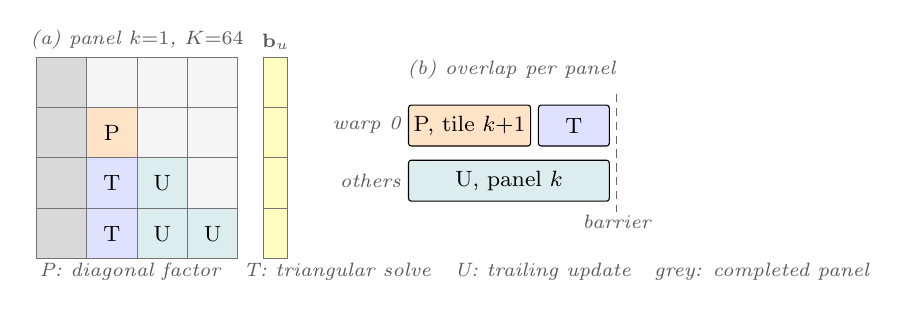
\begin{tikzpicture}[
    font=\footnotesize,
    >={Stealth[length=3pt]},
    t/.style={draw=black!55, minimum size=6.4mm, inner sep=0pt, line width=0.4pt},
    potrf/.style={t, fill=orange!22},
    trsm/.style={t, fill=blue!12},
    upd/.style={t, fill=teal!14},
    idle/.style={t, fill=black!4},
    lane/.style={draw, rounded corners=1pt, minimum height=5.2mm, inner sep=1pt, line width=0.4pt, align=center},
    lbl/.style={font=\scriptsize\itshape, text=black!65, inner sep=1pt}]

% (a) tile view at panel k = 1 of a K = 64 system (4 x 4 tiles of 16 x 16)
\foreach \i in {0,...,3} {
  \foreach \j in {0,...,3} {
    \ifnum\j>\i
      \node[idle] at (0.64*\j, -0.64*\i) {};
    \else\ifnum\j=0
      \node[t, fill=black!15] at (0.64*\j, -0.64*\i) {};
    \else\ifnum\i=1
      \node[potrf] at (0.64*\j, -0.64*\i) {P};
    \else\ifnum\j=1
      \node[trsm] at (0.64*\j, -0.64*\i) {T};
    \else
      \node[upd] at (0.64*\j, -0.64*\i) {U};
    \fi\fi\fi\fi
  }
}
\foreach \i in {0,...,3} {
  \node[t, minimum width=3mm, fill=yellow!25] at (2.72, -0.64*\i) {};
}
\node[lbl, above=0.5mm] at (2.72, 0.32) {$\mathbf{b}_u$};
\node[lbl, above=0.5mm] at (0.96, 0.32) {(a) panel $k{=}1$, $K{=}64$};

% (b) phase overlap between warp 0 and the remaining warps
\begin{scope}[xshift=4.35cm, yshift=-0.2cm]
\node[lbl, anchor=south west] at (0, 0.2) {(b) overlap per panel};
\node[lbl, anchor=east] at (0, -0.35) {warp 0};
\node[lbl, anchor=east] at (0, -1.05) {others};
\node[lane, fill=orange!22, minimum width=15.5mm, anchor=west] at (0.05, -0.35) {P, tile $k{+}1$};
\node[lane, fill=blue!12, minimum width=9mm, anchor=west] at (1.70, -0.35) {T};
\node[lane, fill=teal!14, minimum width=25.5mm, anchor=west] at (0.05, -1.05) {U, panel $k$};
\draw[densely dashed, black!60] (2.70, 0.05) -- (2.70, -1.45);
\node[lbl, anchor=north] at (2.70, -1.45) {barrier};
\end{scope}

% key
\node[lbl, anchor=north west] at (-0.32, -2.25)
  {P: diagonal factor\quad T: triangular solve\quad U: trailing update\quad grey: completed panel};
\end{tikzpicture}

\caption{Tiled blocked Cholesky solver for $K \ge 32$. (a) Tile roles at panel $k{=}1$ of a $K{=}64$ system; the right-hand side $\mathbf{b}_u$ is carried through the panels. (b) Warp~0 factorizes the next diagonal tile while the other warps apply the trailing update of the current panel.}
\label{fig:cholesky}
\end{figure}

\subsection{Execution Pipeline}
\label{ssec:pipeline}

Gram buffers for half a million entities do not fit in device memory, so each half-sweep processes batches of 60{,}000 entities. Gram assembly runs on one CUDA stream, and each finished batch is solved on a second, higher-priority stream using double-buffered Gram storage (lines~\ref{alg:tr:wait}--\ref{alg:tr:solve} of Algorithm~\ref{alg:training}); CUDA events enforce the two true dependencies. On both paths, the harness's RMSE kernel predicts from FP32 factors and reduces in double precision.

\subsection{Convergence Protocol and Fair Comparison}
\label{ssec:protocol}

Both paths follow the same protocol. The factors start from the same seeded $U(0, 0.2)$ initialization, as in cuMF, and $\lambda = 0.048$ throughout. There is no separate validation split: $\lambda$ was selected on the test ratings (Section~\ref{ssec:weightedlambda}), whereas the thresholds and the momentum coefficient were chosen by wall time and stability. Absolute RMSE values may therefore be slightly optimistic; both paths share $\lambda$, so their comparison is unaffected. The train RMSE is evaluated every five sweeps, and training stops when it changes by less than $10^{-3}$ between two checks, with a limit of 50 sweeps. The check interval is thus part of the rule and is fixed.

The baseline is the same binary with a zeroed density array, which routes every entity to the scalar tier and suppresses the WMMA launches. Storage format, batching, solver, RMSE kernel, convergence rule, and stream pipeline are therefore shared. Tile structures are built from training data only, regularization enters only through the solver diagonal, and convergence is judged only on training error. Two restrictions are deliberate. The scalar kernel computes the full $K \times K$ Gram matrix, because a triangular variant ran slower; weakening the baseline was not acceptable. Only $K \in \{16, 32, 48, 64, 96\}$ is supported, because the WMMA shape requires multiples of 16 and each value needs its own register-tile instantiation. Zeroing the density array also disables the FP16 staging inside the scalar kernel, so the two-path ratio covers that optimization as well; Section~\ref{ssec:precisioniso} separates the effects with a single-kernel ablation.

\section{Experimental Evaluation}
\label{sec:eval}

This section compares APR-BALS with its FP32 baseline in a two-path harness that isolates the precision dispatch. Optimizations that apply to only one path, such as momentum, are evaluated in Section~\ref{sec:extended}.

\subsection{Setup and Methodology}
\label{ssec:setup}

Table~\ref{tab:platforms} lists the platforms and datasets. The primary GPU is an RTX~3060 (Ampere); a Tesla~T4 (Turing), accessed through Google Colab, checks portability. All binaries are built from one source tree with \texttt{nvcc -O3} for \texttt{sm\_86} or \texttt{sm\_75}. We use MovieLens 10M, 20M, and 32M \cite{harper2016movielens} and the Netflix Prize data \cite{bennett2007netflix}, each split once at random into 80\% training and 20\% test ratings. Because the split is random, not the Netflix probe set, absolute RMSE is not comparable with leaderboard results.

\begin{table}[!t]
\caption{Execution Platforms and Datasets. Density Is over All Ratings Before the Split}
\label{tab:platforms}
\centering
\footnotesize
\renewcommand{\arraystretch}{1.05}
\setlength{\tabcolsep}{3pt}
\begin{tabular}{lcc}
\toprule
 & \textbf{RTX 3060} & \textbf{Tesla T4} \\
\midrule
Architecture & Ampere, sm\_86 & Turing, sm\_75 \\
SMs, memory & 28, 12 GB & 40, 16 GB \\
FP32 peak (TFLOP/s) & 12.7 & 8.1 \\
FP16 tensor, FP32 acc.\ (TFLOP/s) & 25.5 & 65 \\
CUDA & 12.0, 12.9 & 12 (Colab) \\
\bottomrule
\end{tabular}

\vspace{4pt}

\setlength{\tabcolsep}{2.5pt}
\begin{tabular}{lrrrrr}
\toprule
\textbf{Dataset} & \textbf{Users} & \textbf{Items} & \textbf{Train} & \textbf{Test} & \textbf{Density} \\
\midrule
ML-10M   & 69{,}878  & 10{,}677 & 8{,}026{,}731  & 1{,}973{,}323 & 1.3\% \\
ML-20M   & 138{,}493 & 26{,}744 & 16{,}052{,}927 & 3{,}947{,}336 & 0.54\% \\
ML-32M   & 200{,}948 & 84{,}432 & 25{,}677{,}530 & 6{,}322{,}674 & 0.19\% \\
Netflix  & 480{,}189 & 17{,}770 & 80{,}570{,}989 & 19{,}909{,}518 & 1.2\% \\
\bottomrule
\end{tabular}
\end{table}

Accuracy is the root-mean-square error on the held-out test ratings, and the cost of mixed precision is the relative difference $\Delta = |\mathrm{RMSE}_{\mathrm{APR}} - \mathrm{RMSE}_{\mathrm{base}}| / \mathrm{RMSE}_{\mathrm{base}}$. Speed is reported as the \textit{wall-time speedup}, the ratio of training-loop times from the first sweep to convergence, including RMSE checks. One-time preprocessing, tile construction, and host-to-device transfers, which both paths share, are excluded. Times come from CUDA events on an otherwise idle GPU, and per-stage times from events around every batch.

\textbf{Measurement variability.} Every configuration in Table~\ref{tab:main3060} was run five times in one session, 100 runs in total. The relative standard deviation of the wall-time speedup is at most $0.44\%$ (mean $0.14\%$), and every tabulated speedup reproduces within $0.50\%$. We therefore treat differences below $1\%$ as insignificant. Test RMSE varies by at most $10^{-6}$ across the same runs.

\subsection{Speedup and Accuracy}
\label{ssec:main_results}

Table~\ref{tab:main3060} and Fig.~\ref{fig:speedup_vs_k}(a) report the RTX~3060 results. The baseline and APR-BALS stop after the same number of sweeps in every configuration, so mixed precision does not alter the optimization trajectory. The speedup grows with $K$ because tensor-core efficiency improves with operand width while the scalar baseline's throughput stays nearly flat. On Netflix it rises from $4.07\times$ at $K=16$ to $14.84\times$ at $K=96$. The MovieLens datasets peak at $K=64$ ($11.62\times$ on ML-20M, $11.59\times$ on ML-32M, $10.87\times$ on ML-10M). This peak is real: on ML-20M the $K=64$ and $K=96$ speedups differ by $4.1\%$, ten times the measurement variability.

\begin{table}[!t]
\caption{FP32 Baseline Versus APR-BALS on the RTX 3060. Both Paths Stop After the Same Number of Sweeps (20 on Netflix, 25 on MovieLens). $\Delta$ Is the Relative Test-RMSE Difference in Units of $10^{-3}\%$; APR-BALS Has the Lower RMSE at Every Point. Over Five Repeated Runs, the Relative Standard Deviation of Every Speedup Is at Most $0.44\%$}
\label{tab:main3060}
\centering
\footnotesize
\renewcommand{\arraystretch}{1.02}
\setlength{\tabcolsep}{3.5pt}
\begin{tabular}{llrrrrr}
\toprule
\textbf{Dataset} & & \textbf{$K{=}16$} & \textbf{32} & \textbf{48} & \textbf{64} & \textbf{96} \\
\midrule
\multirow{4}{*}{Netflix}
 & base (s)       & 4.83 & 14.39 & 31.76 & 74.18 & 154.42 \\
 & APR (s)        & 1.19 & 2.00 & 3.13 & 5.34 & 10.41 \\
 & speedup        & 4.07 & 7.21 & 10.14 & 13.90 & \textbf{14.84} \\
 & $\Delta$       & 2.9 & 3.2 & 3.8 & 4.0 & 4.3 \\
\midrule
\multirow{4}{*}{ML-32M}
 & base (s)       & 2.40 & 6.95 & 15.34 & 35.22 & 78.80 \\
 & APR (s)        & 0.54 & 1.00 & 1.69 & 3.04 & 7.28 \\
 & speedup        & 4.43 & 6.94 & 9.07 & \textbf{11.59} & 10.82 \\
 & $\Delta$       & 1.1 & 1.5 & 1.6 & 1.7 & 1.8 \\
\midrule
\multirow{4}{*}{ML-20M}
 & base (s)       & 1.23 & 3.65 & 7.92 & 18.60 & 39.95 \\
 & APR (s)        & 0.30 & 0.54 & 0.90 & 1.60 & 3.58 \\
 & speedup        & 4.08 & 6.76 & 8.83 & \textbf{11.62} & 11.16 \\
 & $\Delta$       & 0.8 & 0.9 & 1.2 & 1.2 & 1.3 \\
\midrule
\multirow{4}{*}{ML-10M}
 & base (s)       & 0.52 & 1.60 & 3.40 & 8.13 & 16.84 \\
 & APR (s)        & 0.13 & 0.25 & 0.42 & 0.75 & 1.61 \\
 & speedup        & 3.93 & 6.42 & 8.16 & \textbf{10.87} & 10.45 \\
 & $\Delta$       & 0.5 & 0.5 & 0.6 & 0.5 & 0.6 \\
\bottomrule
\end{tabular}
\end{table}

\begin{figure}[!t]
\centering
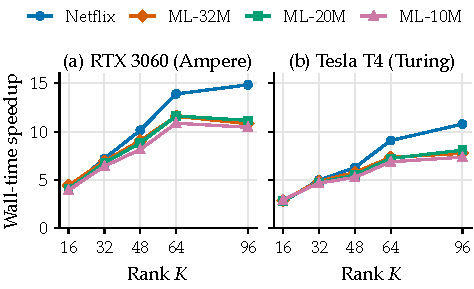
\includegraphics[width=\columnwidth]{figures/fig_speedup.pdf}
\caption{Wall-time speedup of APR-BALS over the FP32 baseline versus latent dimension. }
\label{fig:speedup_vs_k}
\end{figure}

The test-RMSE difference never exceeds $0.0043\%$, and APR-BALS has the lower error at all 20 points. It also has the lower training error, so the effect is not FP16 rounding acting as a regularizer; we have not isolated its cause. The difference grows slowly with $K$ (Netflix: $0.0029\%$ to $0.0043\%$), consistent with the degree-independent error term of \eqref{eq:error_bound}. For scale, raising $K$ from 64 to 96 improves the Netflix test RMSE by $0.19\%$, which is $44$ times larger than the largest precision effect. Test RMSE improves monotonically with $K$ on every dataset, so the most accurate configuration is also the fastest.
\subsection{Cross-Architecture Reproduction}
\label{ssec:t4}

On the Tesla~T4 (Fig.~\ref{fig:speedup_vs_k}(b), single runs, same source and protocol) the speedup is lower but grows with $K$ in the same way, reaching $10.78\times$ on Netflix at $K=96$. The T4's tensor-to-FP32 peak ratio is eight times the RTX~3060's, so peak ratios do not predict the gain of these staging-bound kernels. Accuracy differences stay below $0.007\%$.

\subsection{Where the Time Goes}
\label{ssec:analysis}

Fig.~\ref{fig:stages} breaks the Netflix runs into stages. The baseline's Gram stage sustains 187--280~GFLOP/s, about $2\%$ of FP32 peak, as expected for gather-bound sparse work. APR-BALS raises the same stage to 1.0--11.5~TFLOP/s (both upper bounds). The item side reaches the higher rates because items average more ratings than users, which gives the WMMA kernels longer accumulation loops. Fig.~\ref{fig:stages}(b) shows the consequence. The Gram stage takes 89--96\% of a baseline sweep but only 38--56\% of an APR-BALS sweep, and at $K=96$ the solve becomes the largest stage (48\%), which is why Section~\ref{sec:extended} turns to the solver.

\begin{figure}[!t]
\centering
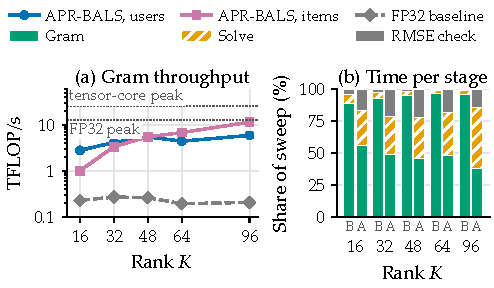
\includegraphics[width=\columnwidth]{figures/fig_stages.pdf}
\caption{Per-stage profile of the Netflix runs on the RTX~3060, both paths of the two-path harness. (a) Gram-stage throughput of APR-BALS per side and of the FP32 baseline (both sides combined), against the peaks of Table~\ref{tab:platforms}. (b) Share of sweep time per stage; under each $K$, bar B is the FP32 baseline and bar A is APR-BALS. Gram time is exposed time, the stage span minus the busy time of the solve that overlaps it, so the throughput in (a) is an upper bound.}
\label{fig:stages}
\end{figure}

\textbf{What limits the tensor-core kernels.} Table~\ref{tab:ncu} lists Nsight Compute counters for the shipped configuration at $K=96$. The dense WMMA kernel uses only $20.5\%$ of the tensor pipe, so it is not bound by tensor throughput. Its most utilized resource is DRAM ($47.6\%$), about twice its SM throughput, which identifies feature-row staging as the limiter. The giant kernel shows the opposite profile ($75.1\%$ SM, $11.4\%$ DRAM), which supports dispatching the two tiers to separate kernels. Their $16\%$ occupancy is deliberate: 240 registers per thread at $K=96$ allow two blocks per SM, and the measured $16.0\%$ matches the predicted $16.7\%$.

\begin{table}[!t]
\caption{Nsight Compute Counters, Netflix $K=96$, RTX 3060. One Steady-State Launch per Kernel; Values Are Percentages of Peak. ``Theor.'' Is the Occupancy Limit Implied by Register Use}
\label{tab:ncu}
\centering
\footnotesize
\renewcommand{\arraystretch}{1.05}
\setlength{\tabcolsep}{2.5pt}
\begin{tabular}{lrrrrrr}
\toprule
 & \textbf{Tensor} & \multicolumn{2}{c}{\textbf{Occupancy}} & & & \\
\textbf{Kernel} & \textbf{pipe} & \textbf{ach.} & \textbf{theor.} & \textbf{SM} & \textbf{DRAM} & \textbf{Regs} \\
\midrule
Dense WMMA Gram       & 20.5 & 16.0 & 16.7 & 25.5 & \textbf{47.6} & 240 \\
Giant WMMA Gram       & 24.3 & 16.6 & 16.7 & \textbf{75.1} & 11.4 & 255 \\
Sparse scalar Gram    & 0.0  & 69.1 & ---  & 29.7 & 42.2 & 64 \\
Cholesky, FP16 tiles  & 0.0  & 54.5 & ---  & 58.4 & 11.0 & 40 \\
\bottomrule
\end{tabular}
\end{table}

\textbf{The solve as the second bottleneck.} In the baseline the solve takes less than $3\%$ of a sweep; in APR-BALS it takes $33$--$41\%$ of the Gram-plus-solve time at $K=16$--$64$ and $56\%$ at $K=96$, and without the blocked solver the $K \ge 48$ speedups would be $28$--$41\%$ lower. The solver is now near a structural floor, launching only $0.96$ waves per SM at $K=96$. A timeline of the shipped binary confirms that the GPU is busy for $99.6\%$ of the run and that the scalar tier accounts for at most $3.2\%$ of wall time, so further gains must come from faster kernels rather than better scheduling.

\subsection{WMMA Kernel Versus Reduced Precision}
\label{ssec:precisioniso}

The two-path comparison changes two things at once: the execution unit and the operand precision. Ampere allows the two to be separated, because WMMA also accepts TF32 operands, which keep the full FP32 exponent range and have eight more mantissa bits than FP16. We built three variants of the Gram stage in one binary, differing by a single compile flag each: the shipped FP16 kernel (\texttt{HMMA.16816.F32}), a TF32 kernel on the same tensor pipe (\texttt{HMMA.1684.F32.TF32}), and the scalar FP32 kernel, selected by raising $\theta_d$ above every entity's degree. Solver, batching, convergence rule, and data are identical. FP16 and TF32 share one dataflow, so their ratio isolates precision. The scalar kernel differs in dataflow as well as execution unit (tiles, full $K \times K$ output, atomic flushes), so its ratio to TF32 measures the WMMA kernel design as a whole; an FP32 CUDA-core kernel with the WMMA dataflow was not built. The giant tier is disabled in all three, because a TF32 giant kernel would exceed the 48~KB static shared-memory limit. The TF32 kernel is inert when disabled; the unmodified build's disassembly is byte-identical.

\begin{table}[!t]
\caption{Precision-Isolating Ablation, Netflix, RTX 3060, Giant Tier Disabled. Milliseconds per Sweep of the Gram Stage Together with the Solve That Overlaps It (Identical in All Three), and the Split of the Total Speedup into a Kernel Factor (FP32 Scalar over TF32) and a Precision Factor (TF32 over FP16). ``Share'' Is $\ln(\text{kernel})/\ln(\text{total})$. All Runs Take 20 Sweeps}
\label{tab:precisioniso}
\centering
\footnotesize
\renewcommand{\arraystretch}{1.05}
\setlength{\tabcolsep}{3pt}
\begin{tabular}{crrrrrr}
\toprule
 & \multicolumn{3}{c}{\textbf{Gram + solve (ms)}} & \multicolumn{3}{c}{\textbf{Decomposition}} \\
\textbf{$K$} & \textbf{FP16} & \textbf{TF32} & \textbf{FP32} & \textbf{Kernel} & \textbf{Prec.} & \textbf{Share} \\
\midrule
16 & 44.4  & 54.3  & 231.4   & 4.26$\times$  & 1.22$\times$ & 87.8\% \\
32 & 70.2  & 82.5  & 695.0   & 8.42$\times$  & 1.18$\times$ & 92.9\% \\
48 & 106.8 & 141.2 & 1549.7  & 10.98$\times$ & 1.32$\times$ & 89.6\% \\
64 & 209.5 & 212.2 & 3647.1  & 17.19$\times$ & 1.01$\times$ & \textbf{99.6\%} \\
96 & 428.8 & 484.7 & 7624.1  & 15.73$\times$ & 1.13$\times$ & 95.7\% \\
\bottomrule
\end{tabular}
\end{table}

Table~\ref{tab:precisioniso} shows that the WMMA kernel, not the reduced precision, produces the gain. At full FP32 range, the TF32 kernel is already $4.3$--$17.2\times$ faster than the scalar kernel, which is $87.8$--$99.6\%$ of the total effect. Moving from TF32 to FP16 adds at most $1.32\times$, and nothing measurable at $K=64$. On ML-20M and ML-10M at $K \in \{32, 96\}$ the kernel share is $92.2$--$96.7\%$, so the result is not specific to Netflix. The small precision factor also confirms the roofline reading: Ampere's TF32 tensor peak is half the FP16 rate, about the FP32 CUDA-core peak, so a throughput-bound kernel would lose about $2\times$, whereas this one loses at most $1.32\times$. For the same reason the $4$--$17\times$ kernel factor cannot come from peak arithmetic rate; it comes from the WMMA kernels' register accumulation, atomic-free output, and triangular work. Accuracy follows the order TF32 $\le$ FP16 $<$ scalar FP32 at every rank, with a total spread of $0.018\%$. Because the measured phase includes the identical solve, every ratio understates the Gram-only effect.

\subsection{Sensitivity and Reproducibility}
\label{ssec:sensitivity}

\textbf{Tier thresholds.} Both thresholds were swept on Netflix at $K=96$ with the shipped binary. The giant threshold is forgiving: over $\theta_g \in \{128, \dots, 2048\}$, a sixteen-fold range that moves between 455 and about 97{,}000 users into the giant tier, wall time varies by only $2.7\%$, and 1024 is the measured optimum. The dense threshold is not. Raising $\theta_d$ from 4 to 8, 16, and 32 increases wall time by $1.05\times$, $1.31\times$, and $2.04\times$, because it moves entities from the tensor cores to the scalar tier. Test RMSE is identical to six decimals and all runs take 20 sweeps. The FP16 staging threshold inside the scalar kernel was not swept.

\textbf{Trajectories and determinism.} On Netflix at $K=32$, the two paths' train RMSE agrees to the fourth or fifth decimal at every checkpoint. The baseline is bit-stable across runs. APR-BALS varies in the sixth decimal because the sparse tail's atomic additions complete in a data-dependent order; the WMMA tiers are deterministic.

\section{Optimizing the Shipped Recipe}
\label{sec:extended}

The two-path harness of Section~\ref{sec:eval} deliberately excludes optimizations that would apply to only one path. This section adds them to form the shipped configuration and measures each step at Netflix $K=96$, where all of them are active. It first justifies the weighted regularizer used throughout.

\subsection{Weighted Regularization}
\label{ssec:weightedlambda}

An early version of this work used a uniform penalty $\lambda I$ with $\lambda = 0.1$. Under it, heavily rated entities are under-regularized as $K$ grows, and the Netflix test RMSE of both paths rose from $0.8607$ at $K=16$ to $1.1929$ at $K=96$. The weighted penalty $\lambda n_u I$ of equ.\eqref{eq:als_update} removes this effect, and test RMSE then falls monotonically ($0.8311$, $0.8233$, $0.8205$, $0.8191$, $0.8176$ for $K = 16$ to 96). Entities without training ratings keep the uniform term to stay positive definite.

The coefficient was selected by a sweep of eight values from $0.010$ to $0.120$ at $K=96$. Both Netflix and ML-20M show a U-shaped error curve with the minimum in $[0.040, 0.048]$. The value $\lambda = 0.048$ is the joint optimum and is used for every result in this paper. It is not optimal for Netflix alone: $\lambda = 0.040$ lowers the Netflix test RMSE by $0.35\%$ ($0.8142$ versus $0.8171$, both with momentum). We kept one protocol-wide value rather than tune per dataset.

\subsection{Narrower-Precision Solver at $K=96$}
\label{ssec:fp16solver}

At $K=96$ the blocked solver is limited by shared-memory capacity (23.1~KB per block). Storing the $K \times K$ factor tiles in FP16, while keeping the right-hand side, diagonal inverses, and all arithmetic in FP32, halves that footprint. Under the uniform penalty this variant is unusable, because heavily rated entities have condition numbers in the hundreds of thousands. Under the weighted penalty the condition number is $O(K/\lambda)$, and the FP16-tile solver reproduces the FP32 solver's test RMSE exactly (Netflix $K=96$: $0.817558$ for both), with no non-finite solves detected by an in-kernel guard. It reduces the solve stage by $23\%$ and total training time from $10.59$~s to $9.44$~s. At $K \le 64$ the variant is not used, because high-degree entities overflow FP16 or the gain is marginal. Since $\kappa u_{16} \approx 1$ at $K=96$, this result is a single measurement, not a general guarantee.

\subsection{Removing Non-Solver Overheads}
\label{ssec:nonsolver}

With the FP16-tile solver in place, an Nsight Systems timeline at $K=96$ shows two non-arithmetic phases taking about a fifth of GPU time: the periodic RMSE check ($16\%$) and a separate pass that adds $\lambda n_u$ to each diagonal ($6\%$). We fused the diagonal update into the solver's load phase, bit-identically. For $K \ge 32$ we replaced the RMSE kernel with a warp-per-entity version that walks the ratings in CSR order and reads the FP16 factor copies already maintained for the tensor cores; the final reported RMSE is still computed in FP32. On Netflix at every rank, runs with and without the fast check stop at the same sweep with bit-identical test RMSE. We also rewrote the giant-tier kernel to stage its loads with asynchronous copies. Measured in the shipped binary, these changes together reduce the Netflix $K=96$ time from $9.35$~s to $7.75$~s ($1.21\times$) with unchanged RMSE. A vendor batched factorization ($2.8\times$ slower than our solver) and a tensor-core formulation of the solve (2.1--2.3~TFLOP/s, launch-bound) were tried and discarded.

\subsection{Momentum Acceleration}
\label{ssec:momentum}

The optimizations above shorten each sweep; momentum reduces the number of sweeps. Near its solution, ALS behaves as a contractive fixed-point iteration, so its factor sequence can be extrapolated with a heavy-ball step: after each solve, $X \leftarrow X_{\text{new}} + \beta (X_{\text{new}} - X_{\text{prev}})$, and likewise for $Y$. The extrapolation term vanishes at a fixed point, so any limit of the extrapolated iteration is a fixed point of ALS; convergence itself is checked empirically. It adds two negligible element-wise kernels per sweep, and $\beta = 0.3$ is used for every dataset and rank. Larger values fail: $\beta = 0.4$ oscillates enough to cancel the savings, and $\beta = 0.5$ makes the factors large enough to overflow the FP16 solver tiles. An in-kernel guard found no non-finite solves at $\beta = 0.3$.

\begin{table}[!t]
\caption{Effect of Momentum ($\beta=0.3$), RTX 3060. All Runs Converge in 15 Sweeps (Without Momentum: 20 on Netflix, 25 on MovieLens). $\Delta$RMSE Is the Change in Test RMSE in Units of $10^{-4}$ (Negative Is Better). ``Total'' Is the End-to-End Speedup of the Shipped Recipe over the FP32 Baseline of Table~\ref{tab:main3060}}
\label{tab:momentum}
\centering
\footnotesize
\renewcommand{\arraystretch}{1.02}
\setlength{\tabcolsep}{4pt}
\begin{tabular}{llrrrrr}
\toprule
\textbf{Dataset} & & \textbf{$K{=}16$} & \textbf{32} & \textbf{48} & \textbf{64} & \textbf{96} \\
\midrule
\multirow{2}{*}{Netflix}
 & $\Delta$RMSE   & $+0.4$ & $-1.7$ & $-3.4$ & $-4.3$ & $-4.1$ \\
 & total          & 5.6$\times$ & 10.1$\times$ & 15.3$\times$ & 21.0$\times$ & \textbf{26.0$\times$} \\
\midrule
\multirow{2}{*}{ML-32M}
 & $\Delta$RMSE   & $-3.9$ & $-4.0$ & $-4.9$ & $-5.3$ & $-4.8$ \\
 & total          & 7.7$\times$ & 11.4$\times$ & 15.9$\times$ & 20.2$\times$ & 21.7$\times$ \\
\midrule
\multirow{2}{*}{ML-20M}
 & $\Delta$RMSE   & $-1.6$ & $-3.7$ & $-5.5$ & $-5.5$ & $-5.4$ \\
 & total          & 7.1$\times$ & 11.1$\times$ & 15.6$\times$ & 20.4$\times$ & 23.2$\times$ \\
\midrule
\multirow{2}{*}{ML-10M}
 & $\Delta$RMSE   & $-0.9$ & $-4.3$ & $-5.8$ & $-5.7$ & $-5.6$ \\
 & total          & 6.7$\times$ & 10.4$\times$ & 14.4$\times$ & 19.1$\times$ & 22.2$\times$ \\
\bottomrule
\end{tabular}
\end{table}

Table~\ref{tab:momentum} shows that every configuration converges in 15 sweeps instead of 20 or 25, a wall-time reduction of $1.30$--$1.33\times$ on Netflix and $1.62$--$1.66\times$ on MovieLens. Test RMSE is equal or better at 19 of the 20 points. The exception is Netflix $K=16$, where it rises by $4.2 \times 10^{-5}$ ($0.831057$ to $0.831099$); five repeated runs confirm this small loss.

\subsection{Cumulative Ablation}
\label{ssec:ablation}

Fig.~\ref{fig:ablation} combines the steps at Netflix $K=96$. The first four bars come from the two-path harness and the last two from the shipped binary, which runs the configuration of the fourth bar in $9.35$~s. The third bar is the FP32-solver reference against which the solver change was measured. It comes from an earlier build of the harness and is $1.7\%$ slower than the second bar, a difference between builds rather than an optimization. The tensor-core dispatch is by far the largest factor ($14.8\times$). The FP16-tile solver and overhead removal together add $1.34\times$ (from $10.41$~s to $7.75$~s), and momentum adds $1.31\times$. Momentum does not depend on precision, so an FP32 baseline could also benefit from it; if the baseline is given the same 15-sweep count, the advantage of the shipped recipe is $19.5\times$ rather than $26.0\times$. We therefore report $14.8\times$ as the effect of the precision dispatch, $19.5\times$ as the iteration-matched advantage, and $26.0\times$ as the end-to-end speedup of the shipped recipe.

\begin{figure}[!t]
\centering
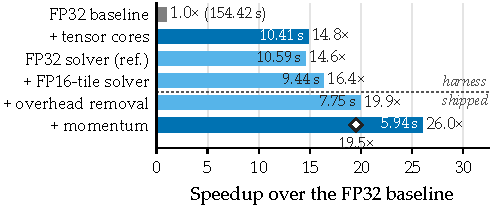
\includegraphics[width=\columnwidth]{figures/fig_ablation.pdf}
\caption{Cumulative ablation at Netflix $K=96$ on the RTX~3060, with wall time inside each bar. Bars above the dashed line come from the two-path harness, and bars below from the shipped binary. The steps follow Sections~\ref{ssec:fp16solver}--\ref{ssec:momentum} in order (overhead removal: fused $\lambda$, fast RMSE check, asynchronous giant-tier copies). The diamond marks $19.5\times$, the advantage if the baseline also stops at 15 sweeps.}
\label{fig:ablation}
\end{figure}

\section{External Validation}
\label{sec:external}

The comparisons so far use a baseline from our own source tree. This section measures the shipped binary against three independently developed GPU systems from different solver families, on the same frozen splits and the same RTX~3060. It then separates the contribution of the tensor-core dispatch from that of the BALS storage format.

\begin{figure*}[!t]
\centering
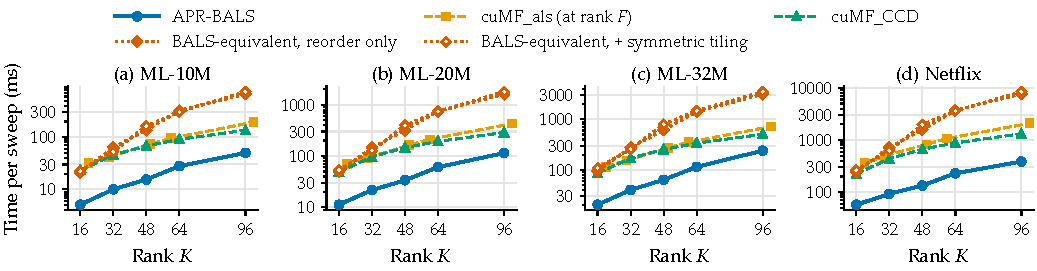
\includegraphics[width=\textwidth]{figures/fig_external.pdf}
\caption{Time per sweep of APR-BALS and three independent GPU systems on the RTX~3060 (log scale). cuMF\_als is plotted at its own rank $F \in \{20, 30, 50, 60, 100\}$, and cuMF\_CCD shows compute time per outer iteration. APR-BALS and cuMF\_als run without momentum. The APR-BALS run with momentum, against which the cuMF\_CCD ratios in the text are computed, is 0.4--2.9\% slower per sweep than the curve shown. The BALS-equivalent kernels are our scalar FP32 reimplementation of BALS (Section~\ref{ssec:balsequiv}).}
\label{fig:external}
\end{figure*}

\subsection{Comparison with cuMF\_als}
\label{ssec:cumfals}

cuMF\_als \cite{tan2016faster} is the most widely cited GPU implementation of explicit-feedback ALS and uses the same weighted regularizer. It supports ranks $F \in \{20, 30, 50, 60, 100\}$, paired here with $K \in \{16, 32, 48, 64, 96\}$, and solves each system with conjugate gradients. By equ.\eqref{eq:gram_flops}, cuMF performs $1.51$, $0.88$, $1.08$, $0.88$, and $1.08$ times the Gram work of APR-BALS per rating at the five pairs, so the pairing favours APR-BALS slightly at two pairs and cuMF at three.

APR-BALS is faster per sweep at all 20 rank pairs, by $3.0\times$ to $6.4\times$ (Fig.~\ref{fig:external}). The margin is widest at $K=16$ ($5.6$--$6.4\times$), where cuMF also does the most extra Gram work. It is narrowest on ML-32M at $K \ge 64$ ($3.0$--$3.1\times$). Training RMSE differs by at most $0.52\%$ at $K \ge 32$, in the direction set by the rank mismatch; at $K=16$, cuMF's 25\% larger rank gives it a $1.4$--$2.2\%$ lower training error.

\textbf{Time to a common target.} Because conjugate gradients may do less work per sweep than an exact Cholesky solve, we also measured the time for each system to reach a common Netflix test RMSE, the worse of the two final values at each rank pair. At four of five pairs the advantage holds or grows ($7.17\times$, $6.15\times$, $6.19\times$, and $5.42\times$ at $K = 32$--96, against $5.38\times$ and $4.64\times$ per sweep at $K=32$ and 64). At $K{=}16$ it falls to $3.16\times$ (versus $6.33\times$), because cuMF's rank-20 model meets the target after 10 sweeps.

\textbf{Held-out accuracy.} On Netflix the two systems agree closely ($0.817559$ for APR-BALS at $K=96$ versus $0.817483$ for cuMF at $F=100$). On the MovieLens datasets cuMF reports a non-finite test RMSE, while its training RMSE stays finite and decreasing. The cause is items without a training rating (cold items), which our split allows (it guarantees one to every user, not every item). Under the weighted regularizer their systems are identically zero, so cuMF's conjugate-gradient step divides zero by zero, and its RMSE kernel's NaN guard is disabled by default; APR-BALS gives such items the uniform term, hence a zero factor. A direct count finds 30, 909, and 4{,}182 such items in ML-10M, ML-20M, and ML-32M, referenced by $0.002\%$, $0.026\%$, and $0.075\%$ of their test ratings, and none in Netflix, the one dataset on which cuMF's value is finite. Predicting zero for these ratings adds $0.02\%$, $0.20\%$, and $0.59\%$ to the APR-BALS test RMSE on the three MovieLens sets. The held-out comparison with cuMF therefore rests on Netflix, and the training-error comparison on all four large datasets.

\subsection{Comparison with cuMF\_CCD and cuMF\_SGD}
\label{ssec:ccdsgd}

The cuMF project also provides cuMF\_CCD, a GPU port of CCD++ \cite{yu2012scalable,nisa2017parallel}, and cuMF\_SGD \cite{xie2017cumf}. We converted each frozen split to their input formats and modified them only to build for sm\_86. cuMF\_CCD runs the same $K$ sweep for 15 outer iterations with its own $\lambda$ (0.05; 0.058 on Netflix). APR-BALS runs the shipped recipe (15 sweeps).

Averaged over the five ranks, APR-BALS is $3.83\times$, $3.72\times$, $3.44\times$, and $4.08\times$ faster than cuMF\_CCD on ML-10M, ML-20M, ML-32M, and Netflix. It is also more accurate at every matched $K$, although cuMF\_CCD uses its own $\lambda$. On Netflix, which has no cold items, the gap is clear ($0.8171$ versus $0.8267$ at $K=96$); on ML-32M it is about the size of the cold-item effect. The margin narrows with rank, from $3.9$--$4.5\times$ at $K=16$ to $2.1$--$3.3\times$ at $K=96$. This is consistent with the cost of a CCD++ sweep growing linearly in $K$ per rating, against quadratically for the Gram stage. BALS reported $2.09\times$, $3.86\times$, and $3.22\times$ over the same system on a TITAN~RTX for ML-10M, ML-20M, and Netflix \cite{chen2021bals}; the platforms differ, so this is not head-to-head.

cuMF\_SGD supports only $k=128$ and so has no curve in Fig.~\ref{fig:external}. Compared with APR-BALS at $K=96$, after 40 epochs it stays above the APR-BALS test RMSE on Netflix ($0.8221$ versus $0.8171$), although it spends less time. On ML-20M and ML-32M it trails by $0.25\%$ and $0.44\%$, comparable to the cold-item effect, and on ML-10M it is $0.08\%$ better and 11\% faster; we claim no accuracy advantage on MovieLens.

\subsection{Tensor Cores Versus the BALS Storage Format}
\label{ssec:balsequiv}

APR-BALS borrows its scalar storage format from BALS, so part of its advantage could come from the format rather than from the tensor cores. To separate the two, we built a faithful scalar-FP32 reimplementation of BALS in a separate binary. It uses the same tiled storage and shared-memory reuse, the frequency reordering of BALS, and, optionally, BALS's symmetric register-tile mapping, with no tensor cores. Both variants reproduce the same training trajectory to six decimals. The BALS runs use an earlier initialization and different sweep counts, so we compare time per sweep.

The two BALS curves in Fig.~\ref{fig:external} yield two findings. First, symmetric tiling does not generalize on Ampere. It speeds up the reorder-only kernel by $1.08$--$1.21\times$ at $K=32$, but it is a net loss at 13 of the 20 dataset--rank pairs (down to $0.77\times$ at $K=48$), with identical sweep counts in both variants. Two opposing costs explain the pattern: idle threads in the triangular mapping ($3.20\times$ the live tiles at $K=16$) and, at $K \ge 48$, a lower occupancy ceiling ($66.7\%$ down to $41.7\%$); only at $K=32$ are both small. Since the scalar kernel is bound by memory access rather than arithmetic, halving its arithmetic should not be expected to pay. This finding concerns BALS's register mapping only, not its storage format or reordering, which both variants retain.

Second, the tensor-core dispatch accounts for most of the advantage over the BALS format, and its share grows with rank. Per sweep, APR-BALS is $4.1$--$4.7\times$ faster than the best BALS variant at $K=16$, $8.8$--$11.8\times$ at $K=48$, and $13.1$--$19.9\times$ at $K=96$; to convergence, the range is $3.5$--$29.9\times$. Because the storage format and reordering are common to both, the per-sweep ratio measures what the WMMA dispatch adds on top of BALS. It includes the host-level overhead removal of Section~\ref{ssec:nonsolver}, whose one separable part, the fast RMSE check, contributes $1.00\times$ at $K=16$ rising to about $1.10\times$ at $K \ge 48$. The rising ratio agrees with the kernel factor of Table~\ref{tab:precisioniso}. Finally, cuMF\_als is faster per sweep than the best BALS variant at $K \ge 32$ ($1.26$--$1.67\times$ at $K=32$), reversing the advantage BALS reported on pre-Ampere GPUs).

\subsection{Threats to Validity}
\label{ssec:threats}

\textbf{Hardware scope.} We tested only an RTX~3060 (Ampere) and a Tesla~T4 (Turing), not data-center parts such as the A100 or H100, whose FP16-to-FP32 throughput ratios and memory bandwidths differ substantially, or non-NVIDIA matrix engines.

\textbf{Problem scope.} Only $K \in \{16, 32, 48, 64, 96\}$ is supported. The restriction follows from the $16 \times 16 \times 16$ WMMA shape; other multiples of 16 need only a new template instantiation and a spill check, and other ranks would need zero padding, which is not implemented. We handle explicit feedback on a single GPU. Implicit-feedback objectives change the Gram structure the dispatch relies on, and multi-GPU partitioning is untested.

\textbf{Measurement limits.} Atomic additions in the sparse tail make APR-BALS reproducible only to about $10^{-6}$ in RMSE, and no claim finer than that is made. Only the two-path wall times (Table~\ref{tab:main3060}) are five-run measurements; the other timings are single runs, the hardware counters are single launches, and the $\lambda$ sweep covers only $K=96$ on two datasets. Finally, the three isolation measures answer different questions: at Netflix $K=96$ the two-path harness gives $14.8\times$ end to end, the kernel ablation $17.8\times$ on the Gram-and-solve phase, and the BALS comparison $19.9\times$ per sweep. None substitutes for another.

\textbf{Baseline and protocol.} The FP32 baseline is slower than cuMF\_als at $K \ge 32$, and the kernel factor of Table~\ref{tab:precisioniso} bundles the tensor pipe with the WMMA dataflow. Convergence is checked every five sweeps, so sweep counts are quantized; the momentum gain and the fixed-iteration \texit{cuMF\_CCD} comparison depend on it.

\section{Conclusion}
\label{sec:conclusion}

This paper has shown that tensor cores can accelerate explicit-feedback ALS on commodity GPUs without measurable loss of accuracy. APR-BALS sorts entities by rating count, sends the dense majority to WMMA kernels with FP16 operands and FP32 accumulation, keeps the sparse tail on scalar FP32 cores, and solves the per-entity systems with a blocked batched Cholesky kernel. Against an audited FP32 baseline that shares its binary, solver, and convergence rule, APR-BALS trains Netflix $4.1$--$14.8\times$ faster on an RTX~3060 for $K=16$--$96$, with test-RMSE differences below $0.005\%$, and reproduces the trend on a Tesla~T4.

The main finding is that the WMMA kernel, even at full FP32 range, accounts for 87.8–99.6\% of the performance gain, while reduced precision provides an additional 1.32× speedup. Further optimizations and momentum raise the end-to-end advantage to $26\times$, and APR-BALS outperforms cuMF\_als and cuMF\_CCD on identical splits. Two results run against expectations: BALS's symmetric register tiling loses on Ampere at most ranks, and the advantage of the tensor-core dispatch over the BALS format grows with rank. The evaluation is limited to NVIDIA Ampere and Turing GPUs, to explicit feedback on one GPU, and to $K$ values that are multiples of the WMMA tile size. At high rank, the batched solve is the largest remaining cost and is launch-bound. Future work might include BF16 operands, implicit-feedback ALS \cite{hu2008collaborative}, multi-GPU partitioning, and evaluation on data-center GPUs.


\section*{Code and Data Availability}
The CUDA implementation, preprocessing and benchmarking harness, and run scripts are publicly available at \url{https://github.com/hafizr283/Baseline_Comarison_Of_APR_BALS} (commit \texttt{9d88f84}), together with the raw logs behind every reported number. The MovieLens datasets are available from GroupLens \cite{harper2016movielens}; the Netflix Prize data \cite{bennett2007netflix} are no longer distributed by Netflix but remain available from public archives such as Kaggle. Seed: 42. Toolchain: CUDA 12.0 and driver 580.159.03 (July runs), CUDA 12.9 and driver 580.173.02 (August runs, which reproduce Table~\ref{tab:main3060} within $0.5\%$), Nsight Compute 2025.2, Nsight Systems 2025.1.

%\section*{Author Contributions}
%M.~H.~Rahman designed and implemented the APR-BALS system, its tensor-core and scalar kernels, the batched Cholesky solvers, and the measurement harness; ported and ran the external baselines; performed all experiments; and drafted the manuscript. K.~M.~A.~Hasan supervised the work, guided the problem formulation and evaluation methodology, and revised the manuscript. M.~M.~H.~Opi contributed to the algorithmic design of the solver and dispatch, advised on the experimental protocol, and revised the manuscript. All authors approved the final version.

%\section*{Acknowledgments}
%This work was carried out in the Department of Computer Science and Engineering, Khulna University of Engineering \& Technology (KUET), Khulna, Bangladesh.

\bibliographystyle{IEEEtran}
\bibliography{ref}

\ifsubmission\else
%\begin{IEEEbiography}[{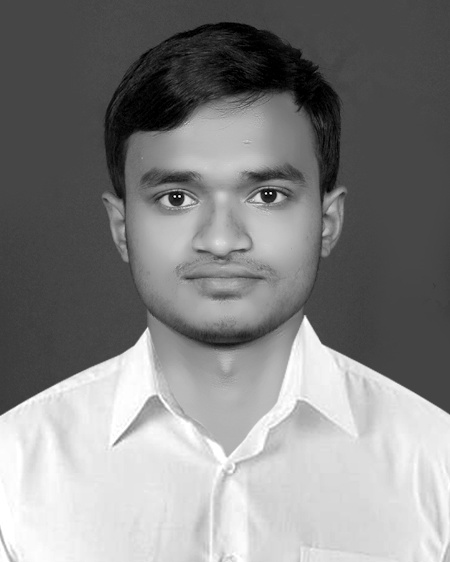
\includegraphics[width=1in,height=1.25in,clip,keepaspectratio]{authors/bio_rahman}}]{Md. Hafizur Rahman}
%received the B.Sc. degree in computer science and engineering from Khulna University of Engineering \& Technology (KUET), Khulna, Bangladesh. His research interests include GPU computing, high-performance parallel algorithms, mixed-precision numerical methods, and recommender systems.
%\end{IEEEbiography}

%\begin{IEEEbiography}[{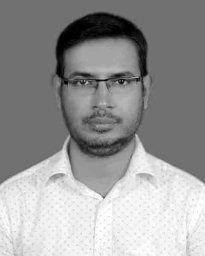
\includegraphics[width=1in,height=1.25in,clip,keepaspectratio]{authors/bio_hasan}}]{K. M. Azharul Hasan}
%received the B.Sc.\ (Engg.) degree in computer science from Khulna University, Bangladesh, in 1999, the M.E.\ degree in computer science from the Asian Institute of Technology (AIT), Thailand, in 2002, and the Ph.D.\ degree from the Graduate School of Engineering, University of Fukui, Japan, in 2006. He is currently a Professor with the Department of Computer Science and Engineering, Khulna University of Engineering \& Technology (KUET), Khulna, Bangladesh. His research interests include data engineering, natural language processing, information retrieval, and high-performance computing.
%\end{IEEEbiography}

%\begin{IEEEbiography}[{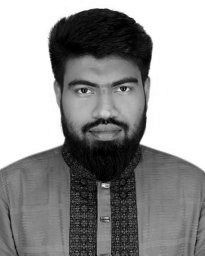
\includegraphics[width=1in,height=1.25in,clip,keepaspectratio]{authors/bio_opi}}]{Md. Mehrab Hossain Opi}
%is an Assistant Professor with the Department of Computer Science and Engineering, Khulna University of Engineering \& Technology (KUET), Khulna, Bangladesh. He was a World Finalist of the International Collegiate Programming Contest (ICPC) in 2024. His research interests include algorithm design, high-performance computing, and data management.
%\end{IEEEbiography}
\vfill
\fi

\end{document}
